\documentclass[letterpaper,12pt,oneside]{book}
\usepackage[top=1in, left=1.25in, right=1.25in, bottom=1in]{geometry}
\usepackage{bachelorstitlepageUNAM}

\usepackage{fancyvrb}

%%%%%%%%%%%%%%%%%%%%%%%%%%%%%
% Comparto una plantilla para la PORTADA que us\'e en mi t\'esis
% basada en el dise\~no gen\'erico que se usa en la Facultad de Ciencias
% Para usarlo \'unicamente aseg\'urate de tener la l\'inea
% \usepackage{bachelorstitlepageUNAM} y el archivo bachelorstitlepageUNAM.sty en el mismo directorio de trabajo.
% y los campos (sin signo %) :
%\author{Nombre del Alumno}
%\title{T\'itulo de la tesis}
%\faculty{Facultad}
%\degree{Grado que obtienes}
%\supervisor{ Tutor}
%\cityandyear{Ciudad y anio}
%\logouni{nombredelescudodelaunamsinespacios}
%\logofac{NombreDeLaImagenDelEscudodeTuFacultadSinEspacios}
% Para sugerencias y comentarios: DM en twitter.com/sglvgdor
% Subir\'e mas adelante la plantilla para maestr\'ia
%%%%%%%%%%%%%%%%%%%%%%%%%%%%%

\author{Pérez Romero Natalia Abigail}
\title{Orquestador para Wireguard minimalista: LinkGuard}
\faculty{Facultad de Ciencias}
\degree{Licenciatura en Ciencias de la Computación}
\supervisor{Dr. José David Flores Peñaloza}
\cityandyear{Ciudad Universitaria, Cd. Mx., 2023}
\logouni{Escudo-UNAM}
\logofac{Escudo-FCIENCIAS}

\usepackage[T1]{fontenc}
\usepackage[utf8]{inputenc}
\usepackage[spanish,es-nodecimaldot,es-tabla]{babel}
\usepackage{graphicx}
\usepackage{tikz}
\usepackage{minted}
% use hyperref to make the table of contents clickable
\usepackage{hyperref}

\graphicspath{{"imagenes/"}}
\usepackage{setspace}
%\usepackage[round]{natbib}

\usepackage{lipsum}

\begin{document}
\frontmatter
\maketitle


\mainmatter

% Crear indice
\tableofcontents

\chapter{Introducción} %

% Introduccion, justificacion y objetivos
En la actualidad, y desde hace tiempo, las empresas al tener una presencia global con múltiples sucursales y empleados remotos requieren establecer conexiones seguras entre sus dispositivos. Para esto hay dos opciones: una línea de alquiler privada y dedicada o compartir una parte del ancho de banda con una línea existente, como Internet. La segunda opción es más económica y flexible, pero menos segura. De ahí surgen las redes privadas virtuales (VPN) que permiten establecer un túnel seguro dentro de una red pública tal como si estuvieran conectados en una red local. Adicionalmente, usuarios finales han encontrado en las VPN una forma de proteger su información y privacidad, además de acceder a contenido restringido geográficamente.

Diferentes protocolos de VPN han sido desarrollados para responder a estos requerimientos, cada uno con sus propias características y funcionalidades, entre ellos OpenVPN y IPsec. Sin embargo, estos protocolos presentan problemas de seguridad, complejidad y rendimiento. Por ejemplo, OpenVPN es un protocolo de VPN de código abierto que utiliza el protocolo SSL/TLS para cifrar el tráfico de red, pero es lento y complejo de configurar. Por otro lado, IPsec es un protocolo de VPN que utiliza el protocolo IKEv2 para establecer un túnel seguro, pero es difícil de configurar y no es compatible con todos los dispositivos.

En respuesta a estos problemas, se ha desarrollado un protocolo de VPN llamado WireGuard que es más simple, más rápido y más seguro que otros protocolos de VPN. WireGuard es más simple que otros protocolos de VPN porque utiliza un enfoque basado en claves públicas para establecer un túnel seguro, en lugar de utilizar certificados SSL/TLS como OpenVPN. WireGuard es más rápido que otros protocolos de VPN porque utiliza un enfoque basado en el kernel para cifrar y descifrar el tráfico de red, en lugar de utilizar un enfoque basado en el usuario como OpenVPN. WireGuard es más seguro que otros protocolos de VPN porque utiliza un enfoque basado en claves públicas para establecer un túnel seguro, en lugar de utilizar un enfoque basado en contraseñas como IPsec.

Si bien WireGuard es un protocolo de VPN simple, la mayor de sus desventajas es la configuración de los pares dentro de la red. Por ejemplo, si se desea configurar una red privada virtual con 10 pares, se debe configurar manualmente cada par con la dirección IP y la clave pública de cada par. Esto puede ser un proceso tedioso y propenso a errores, especialmente si se desea configurar una red privada virtual con un gran número de pares.

Una solución para esta dificultad es propuesa por Tailscale, el cual es un servicio VPN que hace que sus dispositivos y aplicaciones sean accesibles en cualquier parte del mundo, de forma segura y sin esfuerzo. Este software actúa en combinación con el kernel para establecer una comunicación VPN peer-to-peer o retransmitida con otros clientes utilizando el protocolo WireGuard. Tailscale puede abrir una conexión directa con el peer utilizando técnicas de NAT traversal como STUN o solicitar el reenvío de puertos a través de UPnP IGD, NAT-PMP o PCP. [7] Si el software no consigue establecer una comunicación directa, recurre al protocolo DERP (Designated Encrypted Relay for Packets) proporcionados por la empresa. [6] Las direcciones IPv4 asignadas a los clientes se encuentran en el espacio reservado NAT de nivel operador. Esto se eligió para evitar interferencias con las redes existentes[9] ya que el enrutamiento de tráfico a redes detrás del cliente es posible.

Tailscale es una gran solución para la configuración de pares en WireGuard, pero no es una solución de código abierto. Al ofrecer más funcionalidades que las necesarias para la configuración de pares en WireGuard, Tailscale puede ser una solución costosa para empresas pequeñas o individuos que solo requieren configurar pares en WireGuard. Además, Tailscale no permite a los usuarios tener control total sobre la configuración de pares en WireGuard, ya que la configuración de pares en WireGuard se realiza a través de la interfaz de usuario de Tailscale y no a través de la línea de comandos. Y finalmente, Tailscale aumenta la superficie de ataque de la red privada virtual, ya que no solicita la autenticación al usar un servicio crítico como SSH entre los pares.

Existe una alternativa de código abierto del servidor de control de Tailscale llamado Headscale. El objetivo de Headscale es proporcionar a un servidor de código abierto que puedan utilizar para proyectos y laboratorios. Implementa un alcance estrecho, una sola Tailnet, adecuada para un uso personal o una pequeña organización de código abierto. [10]


Aunque Headscale sea una opción open-source no cuenta con un cliente en el dispositivo final y únicamente permite crear un red privada.

Por lo que en este trabajo se propone el desarrollo de un prototipo open-source de un sistema de control de configuración de pares minimalista usando el protocolo WireGuard, inspirado en Tailscale, el cual se adherirá a los principios de UNIX.

Este prototipo de sistema permitirá automatizar la configuración de pares, mediante:
\begin{itemize}
    \item \textbf{Cliente}: Programa que se ejecutará en el dispositivo final, el cual consiste de:
    \begin{itemize}
        \item \textit{Cliente daemon}: Un servidor que actuará como daemon guardando, actualizando y manteniendo la configuración actual de los pares y el cliente.
        \item \textit{Interfaz de cliente}: Un programa que actuará como interfaz recibiendo instrucciones por CLI e interactuando con el cliente daemon.
    \end{itemize}
    \item \textbf{Servidor Orquestador (LinkGuard)}: Un servidor que se encargará de orquestar y automatizar la configuración de los pares dentro de las redes privadas.
\end{itemize}


Se espera que este prototipo automatice la configuración de los pares en una VPN WireGuard, permitiendo que el servidor orquestador actúe como directorio conociendo la dirección IP del endpoint, puertos, llaves públicas, lista de IPs permitidas por cada par en cada red privada. También permitirá la comunicación entre dispositivos finales que no pueden comunicarse directamente, ya que actuará como intermediario en la comunicación.

Se espera que este prototipo reduzca la superficie de ataque de la red privada virtual al no realizar más funcionalidad que la orquestación de los pares en WireGuard. 


Para evaluar el prototipo se propondrán tres escenarios con dos dispositivos finales:
\begin{itemize}
    \item \textbf{Todos los dispositivos finales son alcanzables}: Es decir, tanto el orquestador como los dispositivos finales pueden comunicarse entre sí porque están en la misma red o cuentan con IPs públicas. No existen restricciones como firewalls o NATs.
    
    \item \textbf{Uno de los dispositivos es alcanzable}: En este escenario, el orquestador y los dispositivos final pueden comunicarse entre sí, pero uno dispositivo final no tiene una IP pública o está detrás de un NAT. De forma que el orquestador actuará como intermediario en la comunicación.
    
    \item \textbf{Solo el Orquestador es alcanzable}: Los dispositivos finales no pueden comunicarse entre sí directamente, pero pueden comunicarse con el orquestador, que actuará como intermediario en la comunicación.
\end{itemize}


\chapter{Definiciones}
% Definiciones
\section{VPN} %
Las VPN (Virtual Private Network) son una tecnología de red que permite la transmisión de datos a través de una red pública, como Internet, con seguridad y privacidad mediante la creación de un túnel cifrado entre el dispositivo del usuario y el servidor de la VPN. Por túnel cifrado se define una conexión virtual creada entre el dispositivo del usuario y el servidor VPN. El cifrado se lleva a cabo mediante algoritmos de cifrado como \textbf{AES (Advanced Encryption Standard)}, y la integridad de los datos se mantiene mediante \textbf{HMAC (Hashed Message Authentication Code)}. La autenticación asegura que las partes en la comunicación (cliente y servidor) sean quienes dicen ser. Esto se puede hacer mediante certificados digitales, contraseñas o claves compartidas.

\subsection{Protocolos de túneles}

Los \textbf{protocolos de VPN} definen cómo se establece y mantiene este túnel seguro. Algunos de los protocolos más comunes incluyen:
\begin{enumerate}
   \item \textbf{IPSec (Internet Protocol Security)}: Se utiliza para cifrar y autenticar el tráfico a nivel de red (capa 3). Se combina a menudo con otros protocolos como L2TP (Layer 2 Tunneling Protocol) o IKEv2 (Internet Key Exchange version 2).
   \item \textbf{OpenVPN}: Un protocolo de código abierto basado en SSL/TLS que proporciona alta seguridad, flexibilidad y portabilidad. Puede usar cifrado simétrico y autenticación mediante certificados.
   
   \item \textbf{WireGuard}: Un protocolo más reciente y moderno que utiliza criptografía avanzada y tiene un diseño minimalista. Está optimizado para ser más rápido y eficiente que los anteriores.
\end{enumerate}

\subsection{Flujo de operación de una VPN}
\begin{enumerate}
    \item Conexión inicial:
    \begin{itemize}
        \item El cliente (dispositivo del usuario) establece una conexión con el servidor VPN.
        \item Se negocian los parámetros de cifrado, incluyendo el protocolo y las claves de sesión.
        \item El cliente y el servidor se autentican mutuamente utilizando certificados digitales o claves compartidas.
    \end{itemize}

   \item Transmisión de datos
        \begin{enumerate}
            \item Una vez establecida la conexión segura, el tráfico del usuario se encapsula y cifra antes de enviarlo al servidor VPN.
            \item El servidor VPN descifra los datos y los transmite al destino final en Internet. Al regresar, el proceso se invierte.
        \end{enumerate}
    \item Desconexión: Cuando el usuario finaliza la sesión, la conexión entre el cliente y el servidor se cierra, y el túnel seguro se destruye.
\end{enumerate}

\section{WireGuard}
    WireGuard es un protocolo de comunicación y herramienta de software diseñada para implementar VPN, destacándose por su simplicidad, eficiencia y enfoque en la seguridad. Creado por Jason A. Donenfeld y distribuido bajo la licencia GPLv2, es ampliamente utilizado para mantener conexiones seguras en entornos empresariales, IoT y dispositivos con recursos limitados, acceso remoto en redes públicas e implementaciones como túneles VPN en servicios en la nube.  

    En comparación con otras soluciones como OpenVPN o IPsec, WireGuard ofrece una configuración más sencilla y un enfoque en minimizar la superficie de ataque mediante un código base compacto y auditable de aproximadamente 4,000 líneas, lo que mejora la confiabilidad y facilita auditorías de seguridad. Su diseño optimizado para velocidad y bajo consumo de recursos lo hace ideal para dispositivos de baja potencia o redes con alta latencia, aprovechando capacidades del kernel de Linux para reducir la sobrecarga. Además, es compatible con múltiples sistemas operativos, incluidos Linux, Windows, macOS, Android e iOS.  

    WireGuard utiliza algoritmos criptográficos avanzados como ChaCha20 para cifrado, Curve25519 para intercambio de claves, BLAKE2 para hash y Poly1305 para autenticación de mensajes, garantizando seguridad moderna y eficiente. Funciona a nivel de la capa de red (capa 3 del modelo OSI) y adopta un enfoque punto a punto para establecer túneles entre pares.

\subsection{Flujo de Operación}  
   El flujo de operación de WireGuard comienza con la inicialización, donde se configura una interfaz virtual con una clave privada única, se asocian las claves públicas de los \textit{peers} con sus direcciones IP correspondientes, y se establecen reglas de enrutamiento que redirigen los paquetes a través de la interfaz \texttt{wg0}. En el envío de un paquete, el dispositivo genera el paquete de datos y lo dirige a la interfaz WireGuard, que verifica las reglas de enrutamiento para determinar la clave pública del \textit{peer} de destino. Luego, los datos se cifran usando \texttt{ChaCha20} con claves derivadas del último \textit{handshake}, se encapsulan en un datagrama UDP y se envían al puerto del \textit{peer} especificado. Al recibir un paquete, el dispositivo escucha en el puerto UDP configurado, valida la autenticidad del paquete utilizando \texttt{Poly1305}, descifra los datos con la clave compartida y el \textit{nonce}, y reinyecta el paquete descifrado en la pila de red del sistema operativo como un paquete local.
  
   WireGuard no utiliza un canal de control persistente, lo que le permite operar sin mantener una conexión activa constante; los pares pueden enviar paquetes en cualquier momento. Además, si un \textit{peer} no ha enviado tráfico durante un periodo prolongado, el protocolo renegocia automáticamente el \textit{handshake} en el siguiente envío de paquetes.
   
   \subsection{Algoritmos Criptográficos}  
   Utiliza \texttt{ChaCha20} para cifrar datos, optimizado para hardware sin aceleración AES, y \texttt{Poly1305} para autenticar mensajes y garantizar la integridad de los paquetes. El intercambio de claves se realiza mediante \texttt{Noise Protocol Framework} basado en \texttt{X25519}, permitiendo un intercambio rápido y seguro. Para la derivación de claves seguras emplea \texttt{HKDF} (HMAC-based Extract-and-Expand Key Derivation Function), mientras que la prevención de ataques de repetición se logra mediante un contador de \textit{nonce} monotónico por paquete. Durante el \textit{handshake} inicial, los pares intercambian mensajes criptográficos para autenticarse y negociar claves efímeras para la sesión, con rotación periódica de claves de sesión (cada 2 minutos por defecto) para reforzar la seguridad.
   
\section{Tailscale}  
    Tailscale es una solución de VPN basada en el protocolo WireGuard, diseñada para crear redes privadas de tipo malla (mesh) que conectan dispositivos distribuidos de forma segura y sencilla. Utiliza WireGuard para garantizar alta velocidad y seguridad mediante cifrado moderno, permitiendo conexiones directas entre dispositivos (peer-to-peer) siempre que sea posible, o redirigiendo el tráfico a través de un relay (*derp*) en caso de restricciones como firewalls.
    
   Para los usuarios la configuración es simple solo necesitan instalar la aplicación, autenticarse con cuentas como Google, GitHub o Microsoft, y los dispositivos se registran automáticamente en la red privada. Es compatible con múltiples plataformas como Linux, macOS, Windows, iOS, Android y Raspberry Pi
   
   Tailscale incluye una consola de administración basada en la nube para gestionar dispositivos, permisos y accesos, y emplea autenticación segura basada en sistemas como OAuth o SSO, eliminando la necesidad de manejar claves manualmente. Los administradores pueden definir políticas detalladas de acceso para controlar los permisos a nivel de usuarios o dispositivos. Además, los cambios de configuración se propagan automáticamente, reduciendo el mantenimiento necesario. 

\section{NAT}
NAT (Network Address Translation) es un mecanismo utilizado en redes de computadoras para modificar las direcciones IP en los encabezados de los paquetes mientras transitan por un router u otro dispositivo de red. Su principal propósito es permitir que múltiples dispositivos en una red privada compartan una única dirección IP pública, optimizando así el uso de las direcciones IPv4, que son un recurso limitado. NAT opera típicamente en la capa de red (capa 3 del modelo OSI) y puede aplicarse a nivel de dispositivos como routers o firewalls.

Cuando un dispositivo en una red privada envía un paquete hacia Internet, el router con NAT reemplaza la dirección IP de origen (privada) con su propia dirección IP pública antes de reenviar el paquete. Asimismo, registra esta traducción en una tabla para poder revertir el proceso cuando se recibe una respuesta, reemplazando la dirección IP de destino (pública) en los paquetes entrantes con la dirección privada original del dispositivo interno.

Existen diferentes tipos de NAT:

\begin{itemize}
    \item \textbf{NAT estático}: Traduce una dirección IP privada a una única dirección IP pública de manera fija.
    \item \textbf{NAT dinámico}: Asigna direcciones IP públicas de un conjunto de direcciones disponibles a dispositivos internos según sea necesario.
    \item \textbf{PAT (Port Address Translation)}, también conocido como NAT sobrecargado: Traduce múltiples direcciones IP privadas a una única dirección IP pública, diferenciando el tráfico mediante los números de puerto. Este es el método más común y eficiente.
\end{itemize}

NAT introduce varios desafíos, como la dificultad para establecer conexiones entrantes hacia dispositivos internos, ya que no tienen direcciones IP públicas asignadas directamente. Esto se soluciona parcialmente mediante técnicas como el port forwarding, que asigna puertos específicos a dispositivos internos, y el NAT traversal, utilizado por protocolos como STUN, TURN o UPnP.

La NAT ha sido esencial en la era de IPv4 debido a la escasez de direcciones. La adopción de IPv6 eliminara la necesidad de compartir direcciones IP públicas ya que este protocolo ofrece un espacio de direcciones mucho más amplio y elimina. Sin embargo, la NAT sigue siendo una tecnología ampliamente utilizada por su simplicidad, seguridad implícita (al ocultar dispositivos internos) y compatibilidad con sistemas existentes.

\section{Firewall}
Un firewall es un sistema de seguridad, ya sea software o hardware, que actúa como una barrera protectora entre una red confiable y redes externas, como Internet. Su objetivo principal es controlar y filtrar el tráfico de red según un conjunto de reglas predefinidas, permitiendo únicamente el acceso autorizado mientras bloquea o rechaza el tráfico no deseado o sospechoso.

Un firewall analiza los paquetes de datos que entran o salen de una red. Este análisis puede realizarse en diferentes niveles del modelo OSI. En la capa de red (nivel 3), el firewall examina las direcciones IP de origen y destino para determinar si el tráfico es permitido. En la capa de transporte (nivel 4), evalúa los puertos y protocolos utilizados, como TCP, UDP o ICMP. En la capa de aplicación (nivel 7), inspecciona el contenido del tráfico, como solicitudes HTTP, para detectar patrones o comportamientos maliciosos.

Existen distintos tipos de firewalls según su nivel de complejidad y funcionalidad. Los firewalls de filtrado básico de paquetes aplican reglas simples para permitir o bloquear el tráfico. Los firewalls con inspección de estado (stateful inspection) monitorean el estado de las conexiones y permiten únicamente tráfico relacionado con sesiones previamente establecidas. Los firewalls de próxima generación (NGFW) incluyen capacidades avanzadas como inspección profunda de paquetes (DPI), control de aplicaciones, detección y prevención de intrusiones (IDS/IPS) y filtrado basado en identidad de usuario.

Los firewalls también pueden usar diversas metodologías de filtrado. Algunos emplean listas blancas, que permiten tráfico solo desde fuentes autorizadas, o listas negras, que bloquean tráfico de fuentes específicas. Otros aplican reglas más complejas basadas en criterios como rangos de IP, tipos de protocolos o contenido específico. Además, los firewalls que implementan Network Address Translation (NAT) proporcionan una capa adicional de seguridad al ocultar las direcciones IP internas mediante la traducción entre direcciones públicas y privadas.

En cuanto a su implementación, un firewall puede presentarse como un dispositivo hardware dedicado (por ejemplo, Cisco ASA o Palo Alto), software configurado en sistemas operativos como iptables en Linux o Windows Defender Firewall, o incluso como un servicio en la nube ofrecido por proveedores como AWS o Azure.


\chapter{Desarrollo}

\section{Objetivos del programa}

El objetivo principal es desarrollar un prototipo open-source de un sistema de control de configuración de pares minimalista usando el protocolo WireGuard, inspirado en Tailscale y adherido a los principios de UNIX de modularidad, claridad, composición, separación, simplicidad, transparencia, solidez, representación, menor sorpresa, silencio y reparación. Este sistema tiene la finalidad de automatizar la configuración y sincronización de pares en una VPN WireGuard.

Permitirá a los usuarios automatizar la configuración de los pares de una VPN WireGuard mediante un servidor orquestador y un cliente que se ejecutará en el dispositivo final. De forma que el cliente en el dispositivo final recibirá una vez la configuración por CLI de los pares y la mantendrá actualizada gracias a que enviará esta información al servidor orquestador que actuará como directorio conociendo la dirección IP del endpoint, puertos, llaves públicas, lista de IPs permitidas por cada par en cada red privada. Además, el servidor orquestador permitirá la comunicación entre dispositivos finales que no pueden comunicarse directamente, ya que actuará como intermediario en la comunicación.

Finalmente en este trabajo se validara la funcionalidad y robustez del prototipo mediante pruebas en diferentes escenarios, evaluando su impacto en la simplificación de la configuración y gestión de redes VPN WireGuard.

\section{Descripción del orquestrador}
Este prototipo de sistema permitirá automatizar la configuración de pares, mediante:
\begin{itemize}
    \item \textbf{Cliente}: Programa que se ejecutará en el dispositivo final, el cual consiste de:
    \begin{itemize}
        \item \textit{Cliente daemon}: Un servidor que actuará como daemon guardando, actualizando y manteniendo la configuración actual de los pares y el cliente.
        \item \textit{Interfaz de cliente}: Un programa que actuará como interfaz recibiendo instrucciones por CLI e interactuando con el cliente daemon.
    \end{itemize}
    \item \textbf{Servidor Orquestador (LinkGuard)}: Un servidor que se encargará de orquestar y automatizar la configuración de los pares dentro de las redes privadas.
\end{itemize}


\section{Herramientas a utilizar}
\begin{itemize}
    \item \textbf{Lenguaje de programación}: Python 3.13
    \item \textbf{Framework}: Flask 2.0
    \item \textbf{Sistema de control de versiones}: Git
    \item \textbf{Manejo de dependencias}: Poetry
    \item \textbf{Documentación}: Sphinx
    \item \textbf{Pruebas}: Pytest
\end{itemize}

\section{Funcionalidad del orquestrador}
\subsection*{Comandos de la aplicación}
Describo a continuación los comandos y sus parámetros: 
    % Crear una red privada
    \begin{Verbatim}[breaklines=true]
    python3 main.py create_private_network <name> <segment> <mask>
    \end{Verbatim}
    Crea una red privada con los siguientes parámetros:
    \begin{itemize}
        \item \texttt{<name>}: Nombre de la red privada.
        \item \texttt{<segment>}: Segmento de red de la red privada.
        \item \texttt{<mask>}: Máscara de red de la red privada.
    \end{itemize}

    %  Crea un red privada solo con el nombre
    \begin{Verbatim}[breaklines=true]
    python3 main.py create_private_network <name>
    \end{Verbatim}
    Crea una red privada con el nombre proporcionado y asigna un segmento y máscara de red por defecto.
    El segmento por defecto es 10.0.0.0 y la máscara por defecto es 28.

    % Listar las redes privadas
    \begin{Verbatim}[breaklines=true]
    python3 main.py get_private_networks
    \end{Verbatim}
    Lista todas las redes privadas disponibles en el sistema. Identifica las redes existentes y sus identificadores únicos.

    % Add a public IP address
    \begin{Verbatim}[breaklines=true]
    python3 main.py add_public_ip <endpoint_id> <ip>
\end{Verbatim}

    Esta función permite agregar una dirección IP pública al sistema. La dirección IP proporcionada en <ip> será registrada por el orquestador para utilizarla en la configuración de conexiones o redes relacionadas. Es útil cuando se requiere registrar una nueva IP que será utilizada por un cliente o un servidor.
    Esta función requiere el identificador único de un peer o endpoint, que se puede obtener mediante el comando \texttt{get\_endpoints}.

    
    % Query a client's public IP address
    \begin{Verbatim}[breaklines=true]
    python3 main.py query_client_public_ip
    \end{Verbatim}

    Esta función consulta y devuelve la dirección IP pública asociada al cliente que ejecuta el comando. Es útil para identificar dinámicamente la IP pública actual del cliente, especialmente en redes con direcciones asignadas dinámicamente por el proveedor de servicios de Internet.
    
    % Registrar un peer en una red privada
    \begin{Verbatim}[breaklines=true]
        python3 main.py register_as_peer <name> <private_network_id> <client_ip> <client_port>
    \end{Verbatim}
        
    Permite registrar un nuevo \textit{peer} en una red privada específica con los siguientes parámetros:  
    \begin{itemize}
        \item \texttt{<name>}: Nombre asignado al \textit{peer}.
        \item \texttt{<private\_network\_id>}: Identificador único de la red privada.
        \item \texttt{<client\_ip>}: Dirección IP del cliente a registrar.
        \item \texttt{<client\_port>}: Puerto del cliente que se usará para las comunicaciones.
    \end{itemize}
        

    % Obtener la clave pública de un cliente
    \begin{Verbatim}[breaklines=true]
    python3 main.py get_client_public_key
    \end{Verbatim} 
    Recupera la clave pública del cliente que ejecuta el comando, necesaria para autenticar las comunicaciones en redes privadas mediante WireGuard.
    
   
    
    % Inicializar una interfaz WireGuard
    \begin{Verbatim}[breaklines=true]
    python3 main.py init_wireguard_interface <client_ip>
    \end{Verbatim} 
    Configura e inicializa una interfaz WireGuard usando la dirección IP proporcionada. Esto permite que el cliente participe en redes privadas gestionadas por WireGuard.
    
   
    
    % Crear un peer en la configuración de WireGuard
    \begin{Verbatim}[breaklines=true]
        python3 main.py create_peer <public_key> <allowed_ips> <client_ip> <listen_port>
    \end{Verbatim}
        
    Agrega un nuevo \textit{peer} a la configuración de WireGuard con los siguientes parámetros:  
        \begin{itemize}
            \item \texttt{<public\_key>}: Clave pública del \textit{peer} a agregar.
            \item \texttt{<allowed\_ips>}: Rango de direcciones IP permitidas para el \textit{peer}.
            \item \texttt{<client\_ip>}: Dirección IP asociada al cliente.
            \item \texttt{<listen\_port>}: Puerto de escucha configurado para el \textit{peer}.
        \end{itemize}
        
   
    
    % Cerrar sesión o terminar una sesión
    \begin{Verbatim}[breaklines=true]
    python3 main.py logout
    \end{Verbatim} 
    Cierra la sesión activa del cliente o usuario. Es útil para garantizar la seguridad del sistema y liberar recursos asociados a la sesión.
    

    % Eliminar una red privada
    \begin{Verbatim}[breaklines=true]
    python3 main.py delete_private_network <private_network_id>
    \end{Verbatim} 
    Elimina una red privada identificada por `<private\_network\_id>`. Este comando elimina todas las configuraciones y peers asociados a la red.
    
    % Eliminar un peer de una red privada
    \begin{Verbatim}[breaklines=true]
    python3 main.py delete_network_peer <private_network_id> <endpoint_id>
    \end{Verbatim} 
    Elimina un peer específico, identificado por `<endpoint\_id>`, de una red privada identificada por `<private\_network\_id>`.
    
    % Editar una red:
    
    % Actualizar el segmento de la red
    \begin{Verbatim}[breaklines=true]
    python3 main.py edit_vpn_segment <private_network_id> <new_segment>
    \end{Verbatim} 
    Modifica el segmento de red de una red privada. Este cambio afecta a todos los hosts conectados a la red y desencadena una actualización en tiempo real.
    
    % Actualizar la máscara de red
    \begin{Verbatim}[breaklines=true]
    python3 main.py edit_vpn_mask <private_network_id> <new_mask>
    \end{Verbatim} 
    Cambia la máscara de red de una red privada. Este cambio también desencadena una actualización en todos los hosts conectados.
    
    % Actualizar el nombre de la red
    \begin{Verbatim}[breaklines=true]
    python3 main.py edit_vpn_name <private_network_id> <new_name>
    \end{Verbatim} 
    Renombra una red privada especificada por `<private\_network\_id>` al nuevo nombre proporcionado en `<new\_name>`.



\section{Componentes del orquestrador}

\subsection{Diagrama de clases}
Para el orquestrador tendremos las siguientes clases:
\begin{figure}[h!]
    \centering
    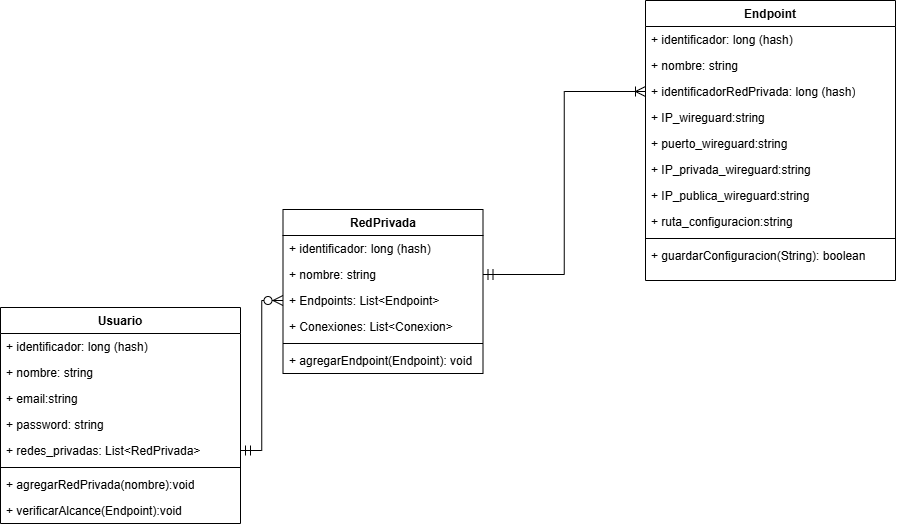
\includegraphics[width=\textwidth]{diagrama-clases.png}
    \caption{Diagrama de clases}
\end{figure}

Bajo la idea de que el orquestrador es el encargado de orquestar la conexión entre los dispositivos finales dentro de una red privada de un cliente, tendremos las siguientes clases:
\begin{itemize}
    \item \textbf{Cliente}: Clase que representa a un cliente que se conecta a la red privada de otro cliente.
    \item \textbf{Endpoiny}: Clase que representa a un dispositivo final que se conecta a la red privada de un cliente.
    \item \textbf{Conexión}: Clase que representa una conexión entre dos dispositivos finales. La idea de esta clase es que el orquestrador sepa que dispositivos finales están conectados entre si y para cuales es necesario relay.
\end{itemize}

\section{Flujo del programa}
El servidor central se encarga de sincronizar los archivos de configuración de la VPN para Wireguard en los nodos de la red.
\subsection{Conexión de dispositivos finales}

Tendremos dos casos en cuando se quieran conectar dos o más dispositivos finales, el primero es cuando es posible que se comuniquen entre si por que tienen direcciones IP ruteables.
El segundo caso es cuando los dispositivos finales no pueden comunicarse entre si por que no tienen direcciones IP ruteables, en este caso el orquestrador deberá ofrecer un mecanismo para que los dispositivos finales puedan conectarse entre sí mediante un relay.
\begin{figure}[h!]
    \centering
    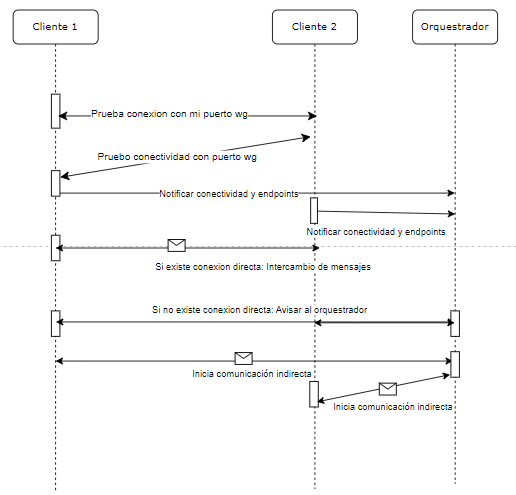
\includegraphics[width=\textwidth]{alcanzabilidad.png}
    \caption{Diagrama de caso de uso: conexión de dispositivos finales}
\end{figure}

\subsubsection{Conexión de dispositivos finales con direcciones IP ruteables. Directa}

En este caso el uno de los clientes se comunica directamente con el otro cliente, el orquestrador deberá enviar un mensaje de confirmación al cliente que solicita la conexión. 
Para esto el cliente A enviara mediante ping al cliente B a la dirección IP y puerto que el orquestrador le proporcionó para la interfaz Wireguard.

Si se obtiene una respuesta entonces consideramos que la conexión fue exitosa (los dispositivos son alcanzables). 
\begin{figure}[h!]
    \centering
    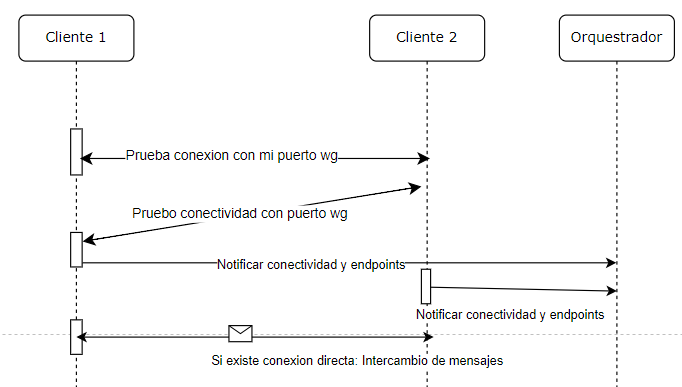
\includegraphics[width=\textwidth]{conexion-directa.png}
    \caption{Diagrama de caso de uso: conexión de dispositivos finales con direcciones IP ruteables. Directa}
\end{figure}


\subsubsection{Conexión de dispositivos finales con direcciones IP no ruteables. Relay}

En este caso el orquestrador deberá ofrecer un mecanismo para que los dispositivos finales puedan conectarse entre sí mediante un relay. 
El cliente A se comunica con el orquestrador para solicitar la conexión con el cliente B, el orquestrador deberá enviar un mensaje de confirmación al cliente A con la dirección IP y puerto del orquestrador, el cliente A deberá enviar un mensaje al orquestrador para que este se comunique con el cliente B. 

\begin{figure}[h!]
    \centering
    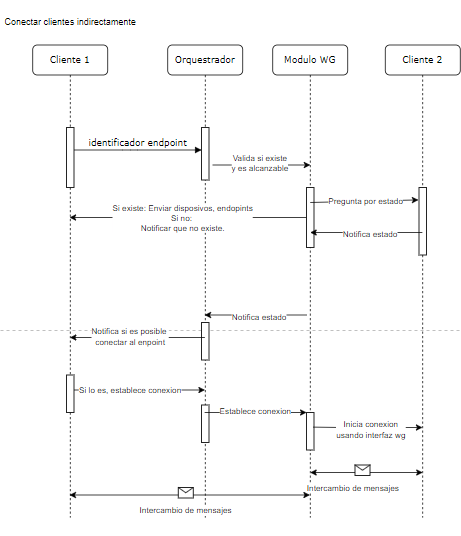
\includegraphics[width=\textwidth]{conecta-clientes-indirectamente.png}
    \caption{Diagrama de caso de uso: conexión de dispositivos finales con direcciones IP no ruteables. Relay}
\end{figure}

\section{Casos de uso}
\subsubsection{Registro de usuario}

En el registro del usuario se deberá solicitar al usuario su nombre, correo electrónico y contraseña, que será enviada al orquestrador en texto plano para su registro, si es exitoso el orquestrador deberá enviar un mensaje de confirmación al usuario.

\begin{figure}[h!]
    \centering
    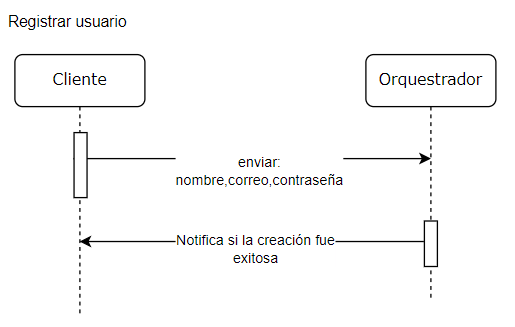
\includegraphics[width=\textwidth]{register-user.png}
    \caption{Diagrama de caso de uso: registro de usuario}
\end{figure}

\subsection{Identificación del usuario}
En esta primera version no nos preocuparemos de que la información del usuario se transmita de forma segura, por lo que el usuario deberá identificarse con un nombre de usuario, correo electrónico y contraseña. Que será enviada al orquestrador en texto plano para su verificación.

\begin{figure}[h!]
    \centering
    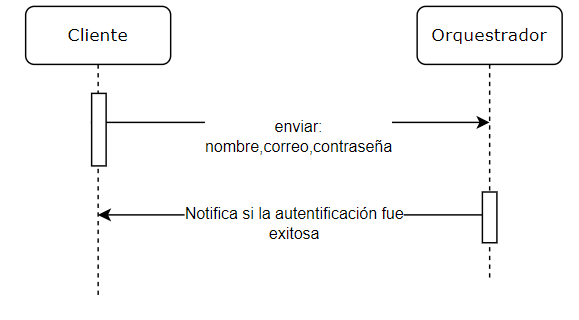
\includegraphics[width=\textwidth]{login-user.png}
    \caption{Diagrama de caso de uso: identificación del usuario}
\end{figure}


\subsection{Registro de una red privada}

Deseamos que el usuario pueda registrar las redes privadas a las que desea conectarse, para ello se deberá implementar un mecanismo de registro de redes privadas.
El cliente deberá enviar un mensaje al orquestrador con el nombre de la red privada que desea crear, si la red privada existe el orquestrador deberá notificar al cliente, si la red privada no existe, el orquestrador deberá crearla y enviar un mensaje de confirmación con la información siguiente: IP asignada, rango, mascara de la red privada creada.

\begin{figure}[h!]
    \centering
    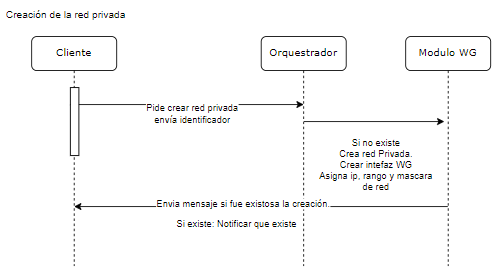
\includegraphics[width=\textwidth]{create-network.png}
    \caption{Diagrama de caso de uso: registro de red privada}
\end{figure}

Una red privada desde el punto de vista del orquestrador es un objeto que contiene la siguiente información:
\begin{itemize}
    \item Identificador
    \item Nombre de la red privada
    \item Lista de dispositivos finales
    \item Lista de conexiones
\end{itemize}

La idea es crear este objeto para almacenar y consultar datos sobre sobre las redes privadas de un cliente.
Luego el razonamiento tras crear un interfaz virtual de Wireguard es que en caso de que la comunicación entre los dispositivos finales no sea posible, el orquestrador pueda actuar como relay dentro de la red privada virtual.


\subsection{Registro de un dispositivo final}
Uno de los objetivos del orquestrador será registrar los dispositivos finales conectados a la red privada, para ello se deberá implementar un mecanismo de registro de dispositivos.

\begin{figure}[h!]
    \centering
    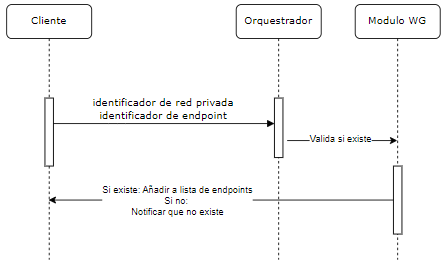
\includegraphics[width=\textwidth]{registro-endpoint.png}
    \caption{Diagrama de caso de uso: registro de dispositivo final}
\end{figure}

El cliente enviara al orquestrador el identificador de la red privada y el dispositivo final que desea registrar.
El orquestrador deberá validar que la red privada exista y que el dispositivo final no esté registrado en la red privada, si es así el orquestrador deberá registrar el dispositivo final y enviar un mensaje de confirmación al cliente.

El orquestrador sera quien asigne la IP de los dispositivos finales dentro de una red privada de los clientes. Así que tambien deberá asignar el rango y la mascara de la red privada. 

\newpage
\subsection{Cliente verifica conectividad con sus endpoint registrados}
El cliente deberá informar al orquestrador si es posible que se comunique con los demás dispositivos finales de la red privada, para ello deberá enviar un mensaje al orquestrador para conocer que dispositivos finales supone que están conectados a la red privada.
Luego este cliente verificara si alcanza a los demás dispositivos finales de la red, mediante un mensaje enviado desde la interfaz Wireguard, es decir, usando las IP asignadas por el orquestrador.

Este caso de uso se deberá hacer con cierta periodicidad, para que el cliente pueda tener información actualizada de la red privada. Y en caso de que el orquestrador la solicite el cliente tendrá la información de la red privada actualizada.

\begin{figure}[h!]
    \centering
    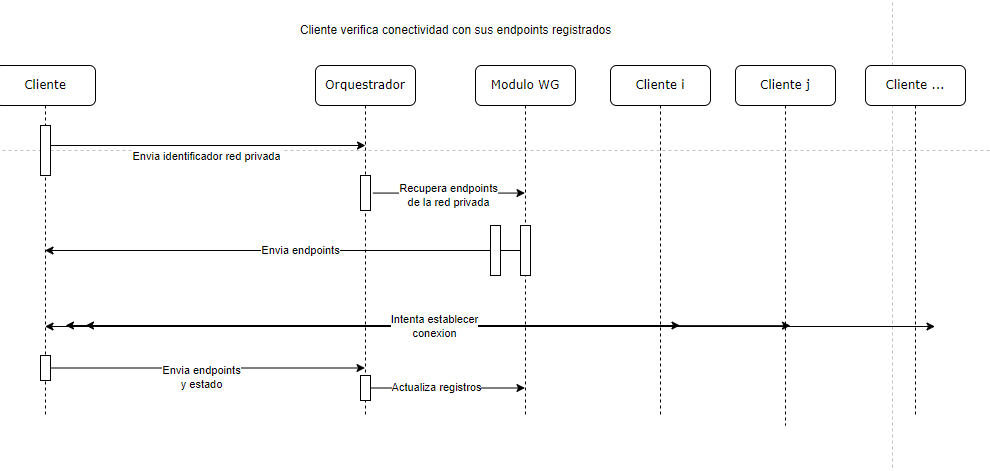
\includegraphics[width=\textwidth]{cliente-alcanza-endpoints.png}
    \caption{Diagrama de caso de uso: cliente verifica conectividad con sus endpoint registrados}
\end{figure}

\newpage
\subsection{Cliente consulta información de red privada al orquestrador}
El cliente deberá poder consultar la información de la red privada a la que está conectado, para ello deberá enviar un mensaje al orquestrador con el identificador de la red privada, el orquestrador deberá responder con la información de la red privada.

\begin{figure}[h!]
    \centering
    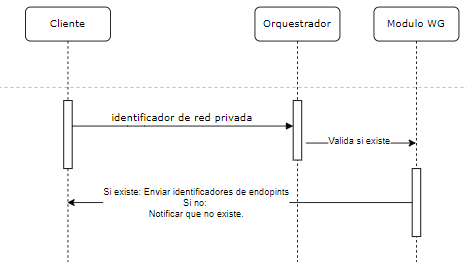
\includegraphics[width=\textwidth]{divulgar-red-privada.png}
    \caption{Diagrama de caso de uso: cliente consulta información de red privada al orquestrador}
\end{figure}


\subsection{Cliente consulta redes privadas disponibles}
El cliente deberá poder consultar las redes privadas disponibles, para ello deberá enviar un mensaje al orquestrador, el orquestrador deberá responder con la lista de redes privadas conocidas.

\begin{figure}[h!]
    \centering
    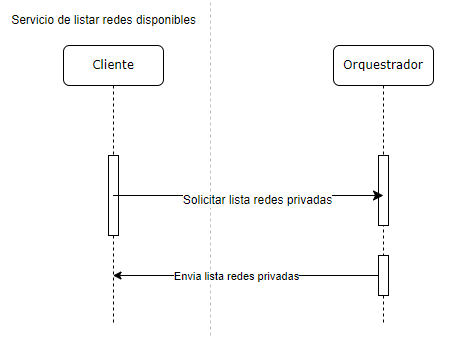
\includegraphics[width=\textwidth]{listar_redes.png}
    \caption{Diagrama de caso de uso: cliente consulta redes privadas disponibles}
\end{figure}

\subsection{Orquestrador divulga tablero de red privada}
Si el cliente envia una solicitud del estado de una red privada al orquestrador, este deberá responder con un tablero de la red privada, que contiene la información de los dispositivos finales conectados a la red privada, las conexiones entre los dispositivos finales y la alcanzabilidad de los dispositivos finales desde el punto de vista del orquestrador.

Esto se deberá hacer con cierta periodicidad, para que el cliente pueda tener información actualizada de la red privada.

\begin{figure}[h!]
    \centering
    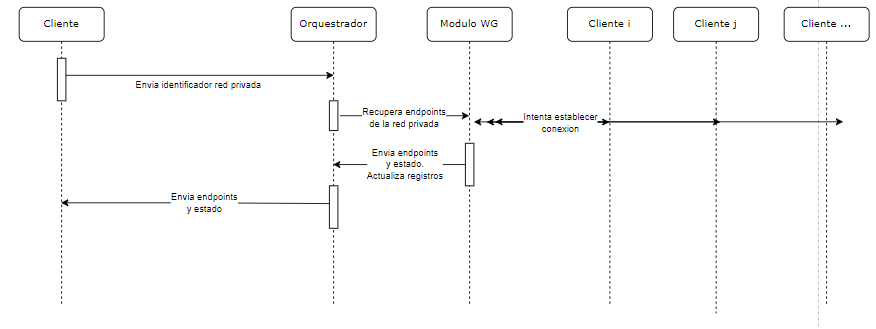
\includegraphics[width=\textwidth]{server-divulga-tablero.png}
    \caption{Diagrama de caso de uso: orquestrador divulga tablero de red privada}
\end{figure}



%\lipsum[1-2]

\chapter{Resultados}  %

Se espera que este prototipo reduzca la superficie de ataque de la red privada virtual al no realizar más funcionalidad que la orquestación de los pares en WireGuard. 


Para evaluar el prototipo se propondrán tres escenarios con dos dispositivos finales:
\begin{itemize}
    \item \textbf{Todos los dispositivos finales son alcanzables}: Es decir, tanto el orquestador como los dispositivos finales pueden comunicarse entre sí porque están en la misma red o cuentan con IPs públicas. No existen restricciones como firewalls o NATs.
    
    \item \textbf{Uno de los dispositivos es alcanzable}: En este escenario, el orquestador y los dispositivos final pueden comunicarse entre sí, pero uno dispositivo final no tiene una IP pública o está detrás de un NAT. De forma que el orquestador actuará como intermediario en la comunicación.
    
    \item \textbf{Solo el Orquestador es alcanzable}: Los dispositivos finales no pueden comunicarse entre sí directamente, pero pueden comunicarse con el orquestador, que actuará como intermediario en la comunicación.
\end{itemize}


\section{Pruebas de Escenario 1. Todos los dispositivos finales son alcanzables}

\begin{itemize}
    \item \textbf{Configuración de la red}: Se configuró un escenario virtual con tres máquinas virtuales, una para el orquestador y dos para los dispositivos finales. Se configuró la red de forma que todas las máquinas virtuales pudieran comunicarse entre sí.
    
    \item \textbf{Conexión entre los dispositivos finales}: Se realizó una conexión entre los dispositivos finales y se verificó que la conexión se realizara correctamente.
    \item \textbf{Pruebas de comunicación}: Se realizaron pruebas de comunicación entre los dispositivos finales para verificar que la conexión se realizara correctamente.
\end{itemize}



\chapter{Conclusiones}  %
\input{conclusiones.tex}

\chapter{Trabajo futuro}  %
\input{trabajo-futuro.tex}

\bibliographystyle{humannat}
%\bibliography{references}

%\backmatter@sglvgdor

% Referencias
%https://www.overleaf.com/learn/latex/Bibliography_management_with_bibtex
\begin{thebibliography}{99}

\bibitem{vpn_comparison}
Abdulazeez, A., Salim, B., Zeebaree, D., y Doghramachi, D. (2020). Comparison of VPN Protocols at Network Layer Focusing on WireGuard Protocol. \textit{International Association of Online Engineering}. Recuperado de https://www.learntechlib.org/p/218341/

\bibitem{linux_network_admin}
Bautts, M., y Dawson, M. (2000). \textit{Linux Network Administrator’s Guide}. O’Reilly Media, 3ra edición.

\bibitem{linux_masquerade}
Bautts, M., y Dawson, M. (2000). \textit{Linux IP Masquerade HOWTO}. Disponible en: \url{https://tldp.org/HOWTO/IP-Masquerade-HOWTO/}

\bibitem{headscale}
Headscale. \textit{An Open Source, Self-Hosted Implementation of the Tailscale Control Server}. Disponible en: \url{https://github.com/juanfont/headscale}

\bibitem{computer_networking}
Kurose, J. F., y Ross, K. W. (2017). \textit{Computer Networking: A Top-Down Approach}. Pearson, 7ma edición.

\bibitem{linux_routing}
Linux Documentation Project. \textit{Linux Advanced Routing and Traffic Control HOWTO}. Disponible en: \url{https://tldp.org/HOWTO/Adv-Routing-HOWTO/}

\bibitem{vpn_protocols}
Narayan, S., Williams, C. J., Hart, D. K., y Qualtrough, M. W. (2015). Network performance comparison of VPN protocols on wired and wireless networks. \textit{2015 International Conference on Computer Communication and Informatics (ICCCI)}. doi:10.1109/iccci.2015.7218077

\bibitem{unix_philosophy}
Basics of the Unix Philosophy. Disponible en: \url{https://cscie2x.dce.harvard.edu/hw/ch01s06.html}

\bibitem{tailscale_derp}
Tailscale. \textit{Terminology and Concepts}. Disponible en: \url{https://tailscale.com/kb/1155/terminology-and-concepts#relay}

\bibitem{tailscale_ip_pool}
Tailscale. \textit{IP Pool}. Disponible en: \url{https://tailscale.com/kb/1304/ip-pool}

\bibitem{tailscale_nat}
Tailscale. \textit{Troubleshooting Device Connectivity}. Disponible en: \url{https://tailscale.com/kb/1411/device-connectivity#nat-types}

\bibitem{tailscale_overview}
Tailscale. \textit{What is Tailscale?} Disponible en: \url{https://tailscale.com/kb/1151/what-is-tailscale/}

\bibitem{nat_traversal}
Tailscale. \textit{How NAT Traversal Works}. Disponible en: \url{https://tailscale.com/blog/how-nat-traversal-works}

\bibitem{wireguard}
WireGuard. \textit{WireGuard: Fast, Modern, Secure VPN Tunnel}. Disponible en: \url{https://www.wireguard.com/}

\end{thebibliography}



\end{document}